\documentclass{standalone}
\usepackage[x11names]{xcolor}
\usepackage{tikz}
\usetikzlibrary{arrows.meta}
\usetikzlibrary{decorations.pathmorphing}
\usetikzlibrary{decorations.pathreplacing}
\tikzset{sdot/.style = {fill, circle, inner sep = 1.5pt}}

\begin{document}
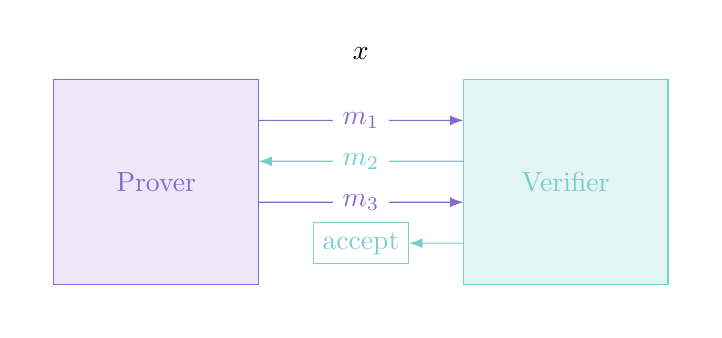
\begin{tikzpicture}[scale = 1.3]
    \draw [white, opacity = 0] (-0.25, -0.25) rectangle (6.25, 2.5);
    \filldraw [fill = MediumPurple3!15, draw = MediumPurple3] (0, 0) rectangle (2, 2);
    \node [MediumPurple3] at (1, 1) {Prover};
    \filldraw [fill = DarkSlateGray3!20, draw = DarkSlateGray3] (4, 0) rectangle (6, 2);
    \node [DarkSlateGray3] at (5, 1) {Verifier};
    \node at (3, 2.25) {$x$};
    \node [MediumPurple3] (m1) at (3, 1.6) {$m_1$};
    \node [DarkSlateGray3] (m2) at (3, 1.2) {$m_2$};
    \node [MediumPurple3] (m3) at (3, 0.8) {$m_3$};
    \node [DarkSlateGray3, draw] (m4) at (3, 0.4) {accept};
    \draw [MediumPurple3, -Latex] (2, 1.6) -- (m1) -- (4, 1.6);
    \draw [DarkSlateGray3, -Latex] (4, 1.2) -- (m2) -- (2, 1.2);
    \draw [MediumPurple3, -Latex] (2, 0.8) -- (m3) -- (4, 0.8);
    \draw [DarkSlateGray3, -Latex] (4, 0.4) -- (m4);
\end{tikzpicture}
\end{document}